%%
% This is an Overleaf template for presentations
% using the TUM Corporate Desing https://www.tum.de/cd
%
% For further details on how to use the template, take a look at our
% GitLab repository and browse through our test documents
% https://gitlab.lrz.de/latex4ei/tum-templates.
%
% The tumbeamer class is based on the beamer class.
% If you need further customization please consult the beamer class guide
% https://ctan.org/pkg/beamer.
% Additional class options are passed down to the base class.
%
% If you encounter any bugs or undesired behaviour, please raise an issue
% in our GitLab repository
% https://gitlab.lrz.de/latex4ei/tum-templates/issues
% and provide a description and minimal working example of your problem.
%%

%\makeatletter
%\def\input@path{{../beamer/}}
%\makeatother

\documentclass[
  german,            % define the document language (english, german)
  aspectratio=169,    % define the aspect ratio (169, 43)
  % handout=2on1,       % create handout with multiple slides (2on1, 4on1)
  % partpage=false,     % insert page at beginning of parts (true, false)
  % sectionpage=true,   % insert page at beginning of sections (true, false)
]{tumbeamer}


% load additional packages
\usepackage{booktabs}
\usepackage{graphicx}
\usepackage{tikz}
\usepackage{url}
\usepackage{pgfplots}
\usepackage{hyperref}
\usepackage{pmboxdraw}
\usepackage{float}
\usepackage{listings}
\usepackage{circuitikz}
%\usepackage[european]{circuitikz}

% image path
\graphicspath{ {./resources/} }

% presentation metadata
\title{Übung 06: Arithmetische und \\sequentielle Schaltungen}
\subtitle{Einführung in die Rechnerarchitektur}
\author{Niklas Ladurner}

\institute{\theChairName\\\theDepartmentName\\\theUniversityName}
\date[\today]{\today}

\footline{\insertauthor~|~\insertshorttitle~|~\insertshortdate}


% macro to configure the style of the presentation
\TUMbeamersetup{
  title page = TUM tower,         % style of the title page
  part page = TUM toc,            % style of part pages
  section page = TUM toc,         % style of section pages
  content page = TUM more space,  % style of normal content pages
  tower scale = 1.0,              % scaling factor of TUM tower (if used)
  headline = TUM threeliner,      % which variation of headline to use
  footline = TUM default,         % which variation of footline to use
  % configure on which pages headlines and footlines should be printed
  headline on = {title page},
  footline on = {every page, title page=false},
}

% available frame styles for title page, part page, and section page:
% TUM default, TUM tower, TUM centered,
% TUM blue default, TUM blue tower, TUM blue centered,
% TUM shaded default, TUM shaded tower, TUM shaded centered,
% TUM flags
%
% additional frame styles for part page and section page:
% TUM toc
%
% available frame styles for content pages:
% TUM default, TUM more space
%
% available headline options:
% TUM empty, TUM oneliner, TUM twoliner, TUM threeliner, TUM logothreeliner
%
% available footline options:
% TUM empty, TUM default, TUM infoline


\begin{document}

\maketitle

\begin{frame}[c]{Feedback}{}
  \begin{center}
    \LARGE  \href{https://t1p.de/wr875}{https://t1p.de/wr875}\\
    
\includegraphics[height=0.5\textheight]{feedback_qr.png}
  \end{center}
\end{frame}

\begin{frame}[c]{}{}
  \begin{center}
    \LARGE  Durchzählen!
  \end{center}
\end{frame}

\begin{frame}[c]{}{}
  \begin{center}
    \LARGE  Keine Garantie für die Richtigkeit der Tutorfolien: Bei Unklarheiten/Unstimmigkeiten
    haben VL/ZÜ-Folien Recht!
  \end{center}
\end{frame}

\begin{frame}[fragile, c]{Besondere Schaltungselemente}{}
  \begin{itemize}
    \item Multiplexer: Leitet Eingang abhängig von Steuersignal durch
    \item ALU (arithmetic logic unit): Recheneinheit eines Prozessors
    \item Latches: Speichereinheit für 1 Bit
    \item Flip-Flops: Taktflankengesteuertes Latch
    \item D-Latch: Data-Eingang und Enable-Eingang
  \end{itemize}
\end{frame}

\begin{frame}[c]{Sequentielle Schaltungen}{}
  \begin{itemize}
    \item Kombinatorische Schaltung: Ausgang ausschließlich durch die Eingänge bestimmt, keine Rückkopplung, keine Abhängigkeit von vorherigen Zuständen
    \item Sequentielle Schaltung: Ausgang abhängig von Eingängen und vorherigem Schaltungszustand, wichtig bspw. für Zähler, Speicher, etc.
  \end{itemize}
\end{frame}

\begin{frame}[c]{Schieberegister}{}
  \centering
  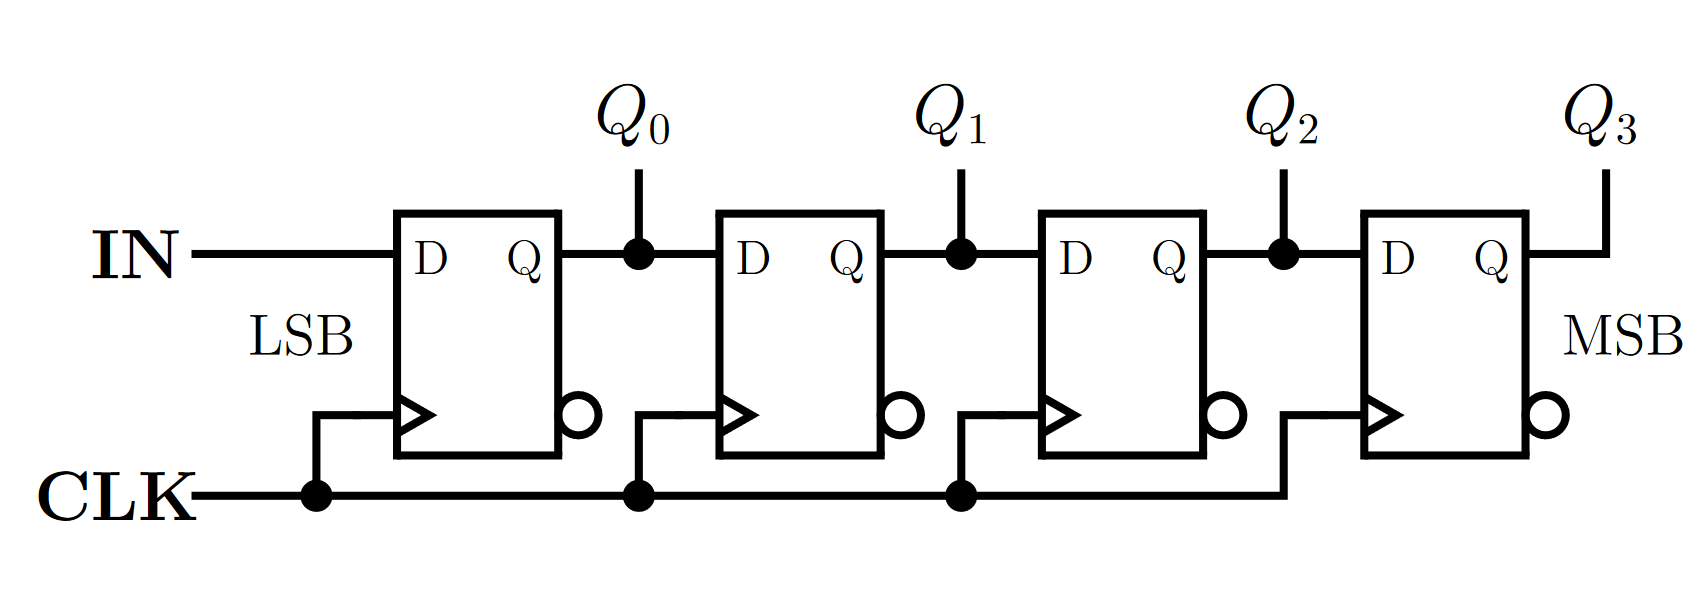
\includegraphics[width=\textwidth]{w06_shift_reg.png}
  \tiny (Das Schieberegister in der Artemis-Hausaufgabe schaut natürlich ein wenig anders aus)
\end{frame}


\begin{frame}[c]{}{}
  \begin{center}
    \LARGE Fragen?
  \end{center}
\end{frame}

\begin{frame}[c, fragile]{Artemis-Hausaufgaben}{}
  \begin{itemize}
    \item H06 - Serieller Multiplizierer bis 03.12.2023 23:59 Uhr
    \item Implementierung von Teilaufgaben in verschiedenen Schaltplänen!
    \item Erklärung Algorithmus siehe \href{https://zulip.in.tum.de/#narrow/stream/1834-ERA---.C3.9Cbungsblatt-06/topic/Vorgehen.20Multiplikation/near/1326249}{hier}
  \end{itemize}
\end{frame}

\begin{frame}[fragile, c]{Links}{}
  \begin{itemize}
    \item Zulip: \href{https://zulip.in.tum.de/#narrow/stream/1917-ERA-Tutorium---Mi-1600-MI4}{\glqq ERA Tutorium - Mi-1600-MI4\grqq}
          bzw. \href{https://zulip.in.tum.de/#narrow/stream/1940-ERA-Tutorium---Fr-1100-MW2}{\glqq ERA Tutorium - Fr-1100-MW2\grqq}
    \item \href{https://de.wikipedia.org/wiki/Schieberegister}{Schieberegister}
    \item \href{https://de.wikipedia.org/wiki/Multiplizierer_(Digitaltechnik)}{Multiplizierer}
    \item \href{https://github.com/logisim-evolution/logisim-evolution/releases}{Logisim Evolution}
  \end{itemize}
\end{frame}

\maketitle

\end{document}
